\section{Programari}
El programari creat en aquest projecte té la finalitat de representar el fractal $f(z) = z^2 + c$, llavors, sabent que necessitarem rapidesa de computació, ja que volem que no vagi massa lent, he utilitzat C++. Aquest llenguatge de programació és un dels més ràpids que existeix actualment. Aquest llenguatge és una ampliació de C derivat a objectes, per tant, la programació és més intuïtiva.

\subsection{Representació de la fractal}
Per a la representació del fractal, utilitzarem una llibreria per a poder mostrar el que estem calculant. Aquesta llibreria es diu olcPixelGameEngine. He escollit aquesta llibreria perquè s'encarregui de la visualització per un simple motiu, que es pot tractar cada píxel per individual. \n
En poder tractar cada píxel com un sol, podem tractar-ho com punts d'un mapa bidimensional. És a dir, cada píxel representa un punt en el pla dels complexos.
\subsubsection{Tractament dels píxels}
Per accedir a cada píxel hem d'anar del 0 al 1920 per als punts d'esquerra a dreta i de 0 al 1080 per als punts de dalt a baix. Això és un problema tenint en compte que la fractal va del $-2$ a l'$1$ i del $-1$ a l'$1$ respectivament. Però aquests números han de ser arbitraris, ja que si volem apropar-nos, aquests canviaran. Per tant, hem d'idear una solució que ho tingui en compte.\n
Bé, per passar de les coordenades de l'ordinador a les de la fractal o a les coordenades que nosaltres volem, hem de normalitzar les coordenades de l'ordinador, perquè vagin de $0$ a $1$ en comptes de $0$ a $1920$ o $0$ a $1080$. Per fer-ho simplement dividirem la coordenada que ens arriba pel nombre total de punts que hi ha. \n
Segon, haurem de saber l'espai que hi ha d'extrem a extrem dins de la fractal. Per saber-ho simplement restarem els extrems per saber la distància i com que ens és igual l'ordre, ho passarem per un absolut perquè ens doni una solució positiva sempre. \n
Finalment, per l'eix de les $x$, agafarem l'extrem de l'esquerra (el més petit) i li sumarem el valor normalitzat multiplicat per l'espai total de les $x$. En el cas de l'eix de les $y$, farem el mateix, però agafarem el valor de dalt i li restarem el valor normalitzat per les $y$ multiplicat per l'espai. \n
Aquesta suma i resta no són arbitràries, la suma la fem perquè els nombres que rebem van d'esquerra a dreta augmentant amb l'eix d'abscisses i volem que vagi igual en la fractal, però van d'amunt en avall en l'eix d'ordenades i en la fractal van a l'inrevés, per això es resta. \n
Haig d'aclarir que aquest tractament només es fa servir en canviar de posició, per al càlcul de la fractal s'utilitza una altra manera igual de vàlida, però canvia una cosa, en l'altre l'hi hem de dir en cada punt on es troba de les coordenades de l'ordinador, en aquesta no. Ja que al principi calcula, restant i fent l'absolut dels extrems i llavors dividint per l'altura o l'allargada de l'ordinador i llavors quan acaba d'una posició suma o resta aquest valor a una variable que ens indica la posició en la qual es troba. Aquesta manera és més directe i computacionalment és una simple suma. \n
Es fan servir les dues, ja que a l'hora de fer el càlcul es necessita rapidesa i a l'hora d'apropar-nos necessitem un punt només.

\subsubsection{Càlcul de la fractal en sí}
Com ja sabem cada punt de la fractal, perquè l'hem calculat en el problema anterior, i també sabem que podem tractar els nombres complexos com a dos nombres, així:
\[z = a + bi\]
\[z = x + yi\]
\centerline{(Sent x, y els valors en cada punt)}
\[z^2 = (x + yi)^2\]
Si ho desenvolupem tenim:
\[z^2 = x^2 + 2xyi + (yi)^2\]
\[z^2 = (x^2 - y^2) + (2xy)i\]
Per tant, sabem quina part del nombre complex serà la real i quina la imaginaria, per tant ho podem desarrollar dient que:
\[z_\mathbb{R} = x^2 - y^2\]
\[z_\mathbb{C} = 2xy\]
Podem fer el mateix per $c$. \n
Així doncs és molt més fàcil de programar, simplement hem de fer unes multiplicacions, sumes i restes. \n
Un cop sabem com determinar cada part, la real i la imaginaria, és hora de calcular-ho. Aquest conjunt, el de Mandelbrot, es calcula posant $z_0 = 0$ i $c$ igual al punt, llavors s'itera un nombre infinit de vegades $z$ en la funció $f(z) = z^2 + c$. Com que no tenim infinit temps, iterarem un nombre finit de vegades i anirem augmentant aquestes iteracions perquè sigui més precís.
\subsubsection*{Determinar quan un punt senvà al infinit}
Per determinar-ho, hem de saber si $|z| > 2$. Aquesta comprovació podem fer-la amb el teorema de Pitàgores:
\[|z| = \sqrt{x^2 + y^2}\]
Per estalviar recursos i no haver de fer l'arrel quadrada cada cop que calculem una iteració d'un punt del pla, farem:
\[|z|^2 = x^2 + y^2 > 2^2\]
Per tant:
\[|z|^2 > 4\]
Quan aquesta inequació es compleixi, deixarem d'iterar el punt i retornarem un valor del 0 al 1, determinat per aquesta operació: $v = k / n$, sent $v$ el valor tornat, $k$ la iteració on ha parat i $n$ el nombre total d'iteracions.\n
En el cas que la inequació no es compleixi i $k = n$ retornarem 0. \n
D'aquesta manera, veurem representat les voreres de la fractal, simplement una decisió artística.
\subsubsection{Dibuix de la fractal}
Per a pinar el fractal simplement accedirem a la matriu on està cada valor $v$ de cada punt i el pintarem. He escollit el color(r, g, b): (255, 163, 119) o \#FFA377, per tant direm que:
\[color_{punt} = (255 - (255 - 255) \cdot v, 255 - (255 - 163) \cdot v, 255 - (255 - 119) \cdot v)\]
\subsubsection*{Resultat inicial}
Si apliquem tot el que hem dit en aquesta part, tindrem el següent resultat:
%Captured_On_Sat_Aug__7_16-05-37_2021-.jpg
\begin{figure}[h!]
    \centering
    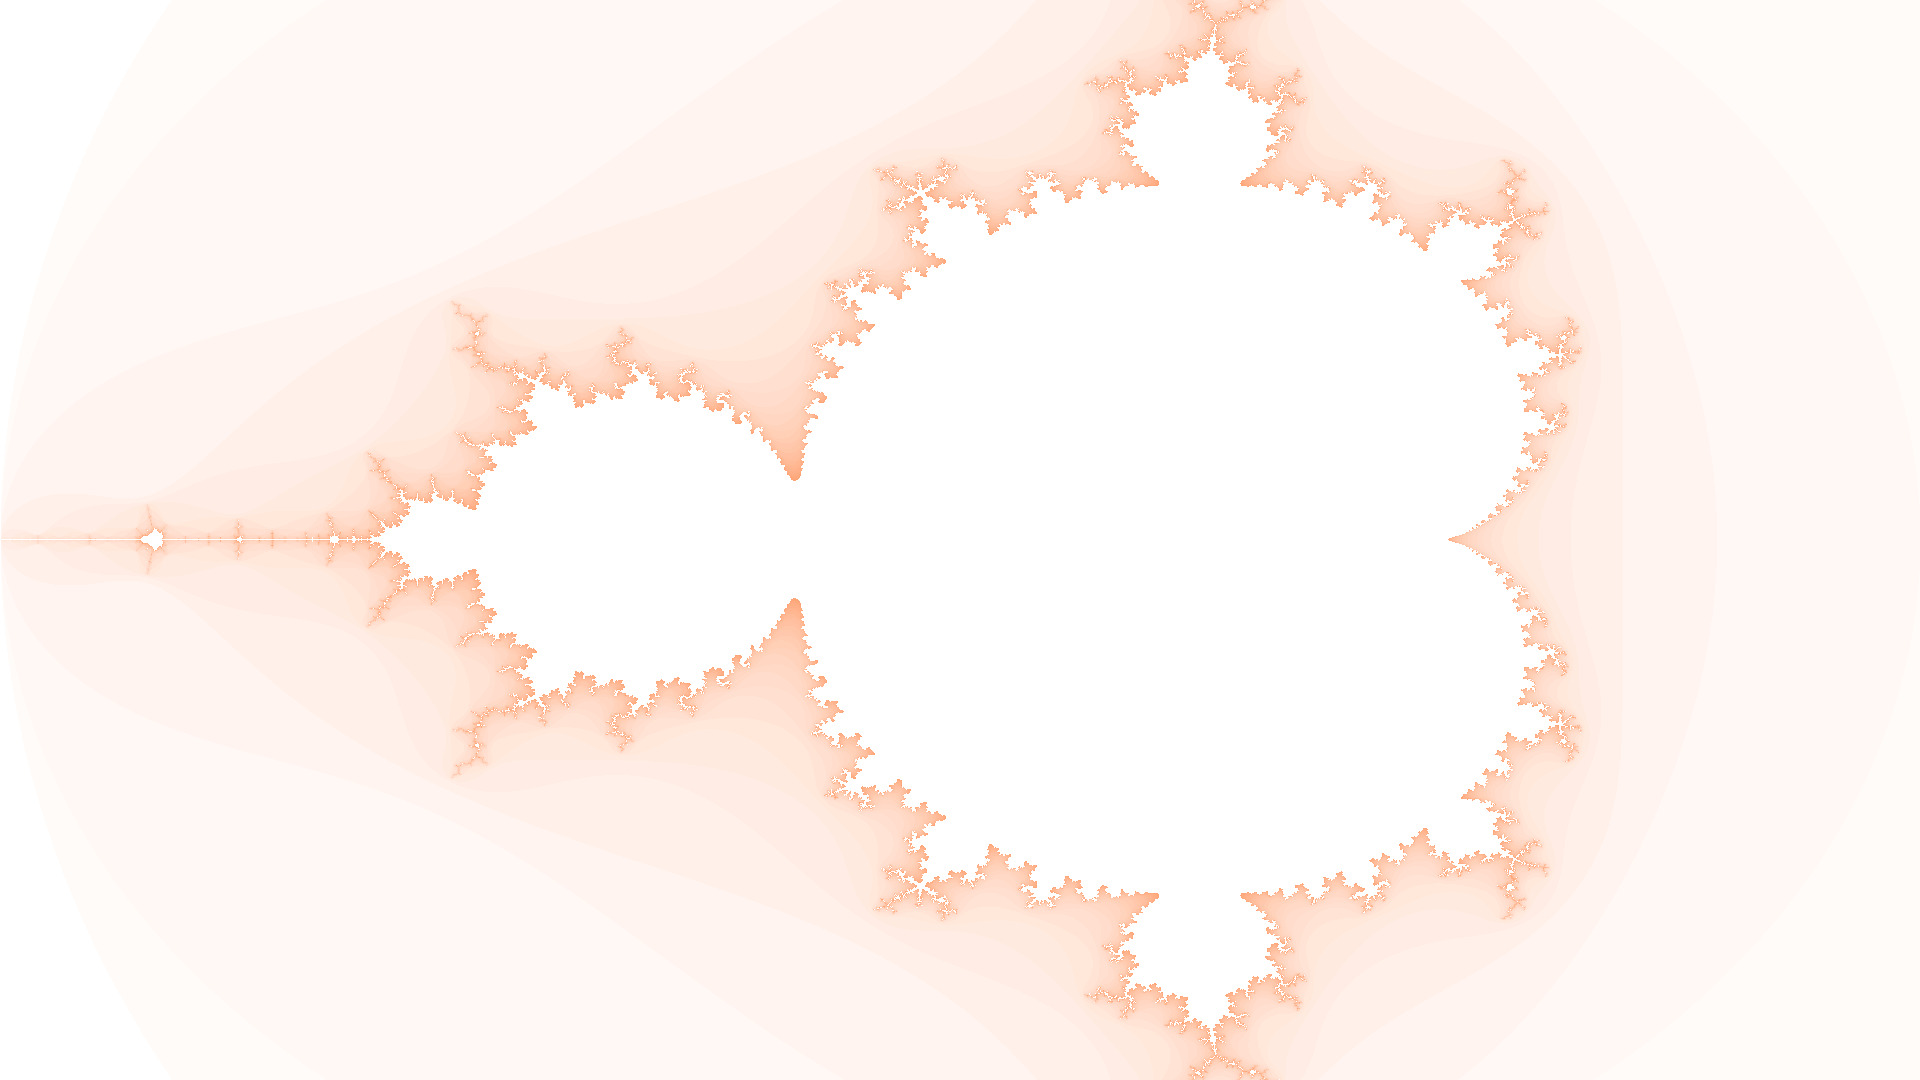
\includegraphics[width=.65\linewidth]{imatges/Captured_On_Mon_Dec__6_18-48-29_2021-.jpg}
    \captionof{figure}{Imatge capturada el 7 d'Agost de 2021 sense ampliacions.}
    \label{fig:resultat_inicial}
\end{figure}
\n \noindent
Jugant amb els colors podem generar imatges com aquesta:
%Captured_On_Sat_Aug__7_16-04-10_2021-.jpg
\begin{figure}[h!]
    \centering
    
\includegraphics[width=.65\linewidth]{imatges/Captured_On_Sat_Aug__7_16-04-10_2021-.jpg}
    \captionof{figure}{}
    \label{fig:jugant_amb_colors}
\end{figure}
\n \noindent
En la figura \ref{fig:jugant_amb_colors}, en comptes de retornar un número del 0 a l'1, es retorna un número del 0 al 255 i se segueix aplicant els colors com hem vist abans, d'aquesta manera, en arribar al número més gran, diguem que multipliquem que ens retorna un dos, en aquest cas es faria (pel blau) $color_{blau} = 163 \cdot 2 = 326$. Aquest és un valor massa gran per aplicar-ho als colors, que van fins al 255. Per tant, es resta 255 al color, és a dir, 71. Llavors, el valor del color blau seria 71.

\subsection{Ampliació}
Per que sigui més interesant el fet de crear aquest programa, farem que pugui ampliar cap a la part que nosaltres volguem. \n
L'ampliació es farà quan l'usuari premi qualsevol punt de la pantalla i arrossegui el cursor fins on vulgui. \n Per a que la tria del lloc sigui més visual, dibuixarem un rectangle al lloc on s'ampliarà. \n
Bàsicament direm, quan el botó esquerra del cursor hagi estat pres, guardarem aquestes coordenades, que aniran de 0 a 1920 i de 0 a 1080, i quan es deixi de premer i estigui a un altre lloc suficientment lluny, a uns 30 píxels, llavors "guardarem" les coordenades finals del cursor.
\subsubsection{Tractament de les coordenades finals del cursor}
"Guardarem" ja que no volem que ens quedi la pantalla estirada: \n
Posar imatge. \n
Perque la pantalla no quedi estirada simplement hem de mantenir l'\emph{Aspect Ratio}. I que és això? Doncs es básicament els píxels d'amplada dividits pels d'altura. L'estandar ara mateix és 16:9, és a dir, per cada 16 píxels que hi ha d'amplada hi ha 9 d'altura. Sabent aquesta definició és senzill doncs saber a quin lloc correspondria l'altura final en relaició a la amplada que estem recorrent amb el cursor. \n
Sabent que la nostra pantalla és de 16:9:
\[\frac{16}{9} = \frac{amplada}{altura}\]
Sabem l'amplada (posició del cursor en X), ens interesa l'altura:
\[altura = \frac{9 \cdot amplada}{16}\]
Doncs ja la tenim. Es senzill.
\subsubsection{Ampliació en sí}
Fent us de la funció que hem creat abans, per saber quina coordenada li correspon al fractal donant-li una coordenada del cursor, li donem els punts que ens han sortit, i, depenent de la posició final del cursor, si està més adalt, més a l'esquerra, més abaix, les igualem a les variables dels límits. \n
Llavors, si fem que just després s'actualitzi la fractal, aquesta s'ampliarà.
